\chapter{Symulacja z zakłóceniem}

\section{Dobranie parametru $D_{z}$}

Ponieważ oba sygnały (sterowanie oraz zakłócenie) są wariacją jednego, tego samego sygnału dobrano dla nich taki sam horyzont dynamiki równy 361 (wyznaczony jako punkt w której wartość odpowiedzi po raz pierwszy przekracza 0,995 maksymalnej wartości dla toru sterowanie-wyjscie - porównywalny horyzont otrzymano prowadząc to samo postępowanie dla toru zakłócenie-wyjscie).

\section {Symulacja z pomiarem zakłóceń}

Symulacja polegała na jednorazowej zmianie wartości zadanej oraz dwukrotnej zmianie wartości zakłóceń. Wyniki symulacji z uwzględnieniem pomiaru zakłóceń przedstawiono na rysunku \ref{zaklocenia}:

\begin{figure}[h!]
	\centering
	\includegraphics[scale=0.8]{Rys/LAB2_DMC_ZAK_ON_N=120Nu=20lambda=0.1error=127.0945tau=1.eps}
	\caption{Symulacja z pomiarem zakłóceń}
	\label{zaklocenia}
\end{figure}
\FloatBarrier

\section {Symulacja bez pomiaru zakłóceń}

Dokonano analogicznego postępowania, jednak wyłączono pomiar zakłóceń (ciągle trafiały do obiektu, jednak regulator nie brał ich pod uwagę przy wyliczaniu sterowania). Wyniki symulacji przedstaiono na rysunku \ref{bez}:

\begin{figure}[h!]
	\centering
	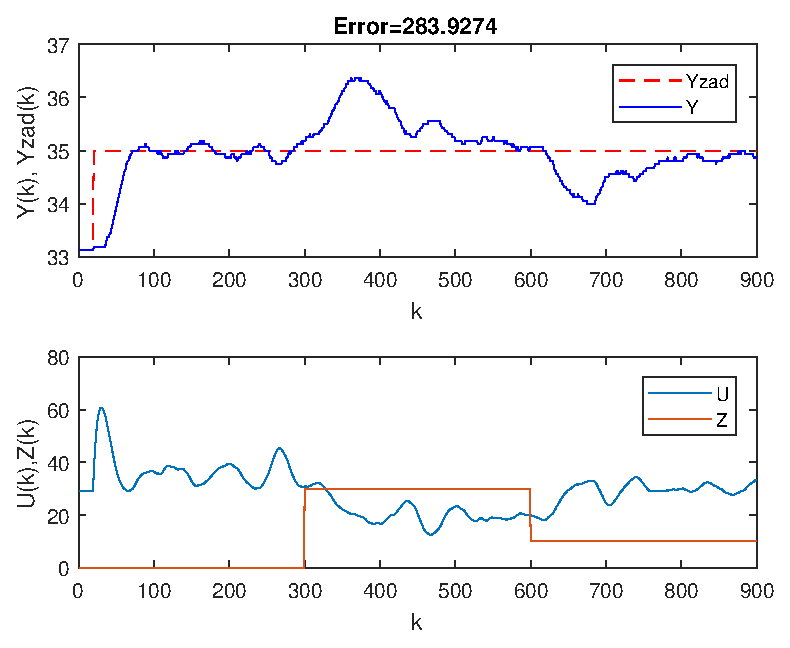
\includegraphics[scale=1]{Rys/LAB2_DMC_ZAK_OFF_N=120Nu=20lambda=0.1error=283.9274tau=1.eps}
	\caption{Symulacja bez pomiaru zakłóceń}
	\label{bez}
\end{figure}

\section {Wnioski}

Zgodnie z przewidywaniami uwzględnienie zakłóceń w regulacji znacznie poprawiło jej jakosć - osiągnięty błąd jest znacznie niższy. 